% latex article template

% cheat sheet(eng): http://www.pvv.ntnu.no/~walle/latex/dokumentasjon/latexsheet.pdf
% cheat sheet2(eng): http://www.pvv.ntnu.no/~walle/latex/dokumentasjon/LaTeX-cheat-sheet.pdf
% reference manual(eng): http://ctan.uib.no/info/latex2e-help-texinfo/latex2e.html

\documentclass[12pt, a4paper]{article}
\title{TDT4171 - Assignment 1}

\PassOptionsToPackage{hyphens}{url}
\usepackage[pdfborder=0 0 0]{hyperref}
\usepackage[utf8]{inputenc}
\usepackage[english]{babel}
\usepackage{graphicx}

% hides the section numbering. 
\setcounter{secnumdepth}{-1}

% Graphics/image lications and extensions. 
\DeclareGraphicsExtensions{.pdf, .png, .jpg, .jpeg}
\graphicspath{{./images/}}

% Author
\author{
        Magnus L Kirø \\
}
\date{\today}

\begin{document}
\maketitle
\pagenumbering{arabic}

\subsection{I}
a) There are 2.598.960 atomic events(different 5-card hands)

b) For exactly each hand the chance of getting that exact one is: 0.000385\%.

c) 
Royal straight flush: 0.000154\%
Four of a cind: 0.0240\%

\subsection{II}
\begin{figure}[htb]
    \centering
    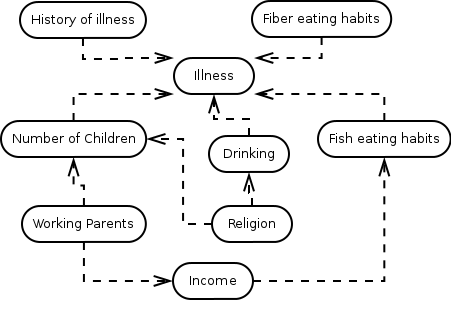
\includegraphics[width=\textwidth]{byesian1}
    \caption{II - Bayesian network}
    \label{II2}
\end{figure}
(See fig: \ref{II2})
Working parents and religion are conditionally independent.
As is fiber eating habit and fish eating habit. 
History of illness and number of children are also conditionally independent. 

This is reasonable because the real life events of these are easily distinguishable and can be related to actual cases, 
proving that these events dosen't affct eachoter. 

\subsection{III}

Probability table: 

a=action, 1=opened door, 2=winning door, 3=first choosen door \\
\begin{tabular}{ l c r }
  door & a1 & a2 \\
  1 & 0.33 & 0 \\
  2 & 0.33 & 0.5 \\
  3 & 0.33 & 0.33 \\
\end{tabular}

Byesian network representing the graph of the choices: \ref{III}
\begin{figure}[htb]
    \centering
    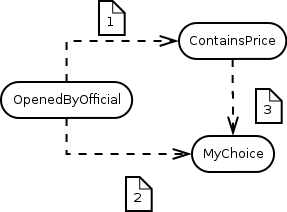
\includegraphics[width=\textwidth]{doors}
    \caption{III - doors}
    \label{III}
\end{figure}

Description to figure: 

1: The price is not behind the door that gets opened, so this changes the probability of the door with the price from 0.33 to 0.5

2: The opening of the door without a price will inflict change in the probability of the players choosen door. 
The choosen door has 0.33 chance of being correct before the opening of one door. This probability remains after the door opening. 

3: When the probability of remining unchoosen door is increased to 0.5.
The choice of doors should also change as the probability of winning is increased from 0.33 to 0.5 

\end{document}
